\section{\textit{Bubble Sort}}

\textit{Bubble Sort} é um dos algoritmos de ordenação mais simples que existe. A ideia dele é iterar sobre uma lista comparando os elementos adjacentes e, caso o primeiro seja maior que segundo, nos fazemos um \textit{swap} (troca), caso queíramos ordenar a lista de forma adjacente.

Apesar de ser o mais simples, não é o mais eficiente. Como estamos comparando elementos adjacentes, nós temos que iterar a lista diversas vezes, comparando os elementos dois-a-dois. Ele é útil em casos onde a lista de elementos não é tão grande.

\subsection{Explicação do Algoritmo}
Nós vamos começar pelo elemento presente no \textit{index} 0 da lista/vetor e vamos comparar com o elemento presente no \textit{index} 1. Caso o primeiro elemento seja maior, nós vamos trocar ele com o segundo elemento. Após isso, nós vamos comparar o elemento do \textit{index} 1 com o elemento no \textit{index} 2. Se for maior, trocamos, caso contrário, apenas seguimos com o algoritmo. A imagem abaixo ilustra melhor essa ideia.
\begin{figure}[H]
    \centering
    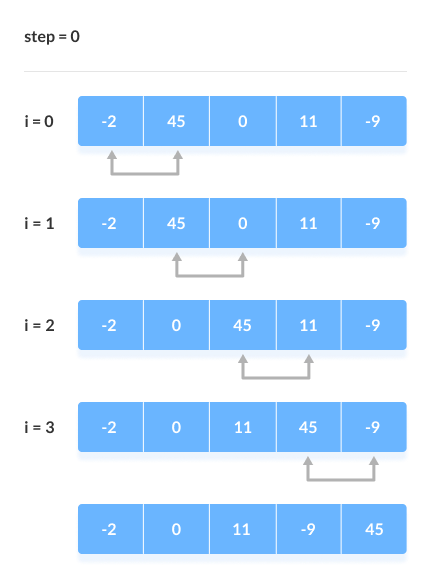
\includegraphics[scale=0.5]{assets/bubble_sort.png}
    \caption{Comparação de elementos adjacentes no \textit{bubble sort}. Fonte: Programiz}
    \label{fig:bubble_sort_0}
\end{figure}

\subsection{Implementação Iterativa}
\begin{lstlisting}[language=C]
void bubbleSort(int* vector, int numberOfElements) {
    while(n > 2) {
        for(int i = 0; i < numberOfElements - 1; i++) {
            if(vector[i] > vector[i + 1]) {
                int aux = vector[i];
                vector[i] = vector[i + 1];
                vector[i + 1] = aux
            }
        }
        numberOfElements--;
    }
}
\end{lstlisting}

\subsection{Implementação Recursiva}
\begin{lstlisting}[language=C]
void bubbleSort(int* vector, int numberOfElements) {
    if (numberOfElements < 2)
        return;
    for(int i = 0; i < numberOfElements - 1; i++) {
        if(vector[i] > vector[i + 1]) {
            int aux = vector[i];
            vector[i] = vector[i + 1];
            vector[i + 1] = aux
        }
    }
    bubbleSort(vector, numberOfElements-1);
}
\end{lstlisting}

\subsection{Pontos Importantes}
\begin{itemize}
    \item O \textit{for loop} vai até numberOfElements - 1 pois dentro do \textit{if} fazemos i + 1. Caso o \textit{loop} fosse até numberOfElements, na última posição teríamos um erro pois tentaríamos acessar uma posição que não existe; 
    
    \item Precisamos criar uma variável \textit{aux} para não perdermos o valor de um dos elementos;
\end{itemize}
